<<<<<<< HEAD
\subsection{Ecualizador de Fase}
=======
empieza el 4

\subsection{Ecualizador de Fase}


\begin{figure}[H]
	\centering
	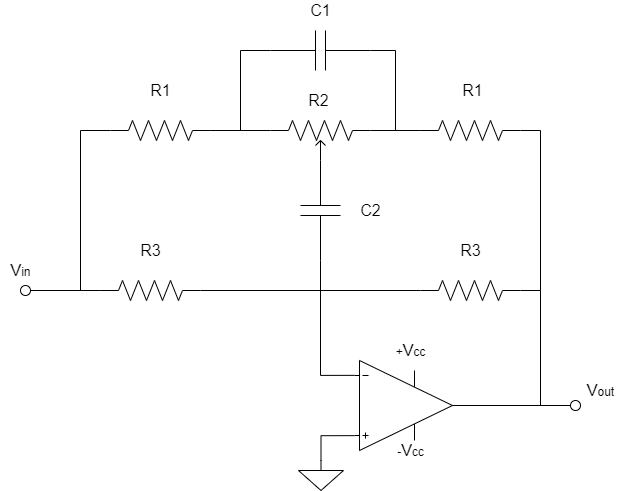
\includegraphics[scale=1]{../Ejercicio4-EcualizadorDeFase/Informe/Ecualizador de Fase.png}
	\caption{Circuito Ecualizador de Fase}
\end{figure}


\subsection{Análisis matemático}

Para analizar el circuito propuesto, se opto por reemplazar la resistencia variable $R_2$ por dos resistencias las cuales llamaremos $R_{21}$ y $R_{22}$, de esta forma será más fácil poder resolver el circuito propuesto, para esto definimos:

\begin{align}
	\begin{equation}
		R_{21} = R_2 . \delta
	\end{equation}
	\begin{equation}
		R_{22}= R_2 . (1 - \delta)
	\end{equation}
\end{align}


\begin{figure}[H]
	\centering
	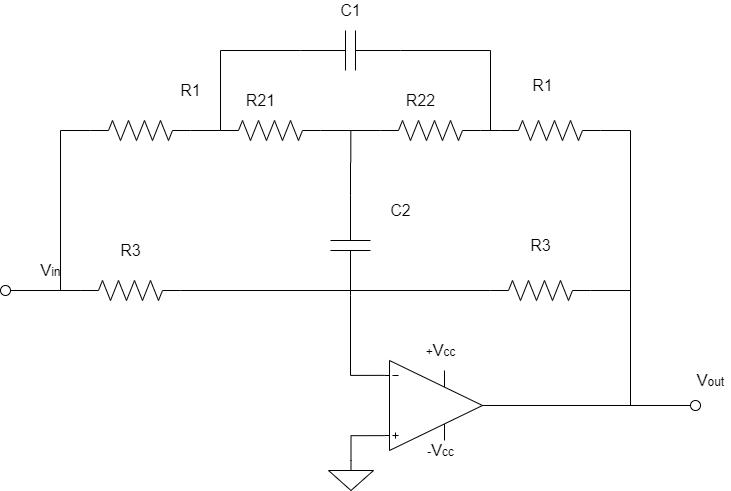
\includegraphics[scale=1]{../Ejercicio4-EcualizadorDeFase/Informe/EcSinPot.png}
	\caption{Modelo matemático}
\end{figure}

Se utilizo el reemplazo de impedancia de configuración triangulo a estrella y luego una transformación de configuración estrella a triangulo como se muestra en las imágenes \ref{1reemplazo} y \ref{2reemplazo}  para poder simplificar el circuito lo mas posible el circuito.
Para el primer reemplazo se usaron las siguientes ecuaciones:

\begin{align}
	\begin{equation}
		Z_{AB}= \frac{1}{sC_1}
	\end{equation}
	\begin{equation}
		Z_{BC}= R_{22}
	\end{equation}
	
	\begin{equation}
		Z_{CA}= R_{21}
	\end{equation}
\end{align}

\begin{figure}[h]
	\caption{1° Reemplazo}
	\centering
	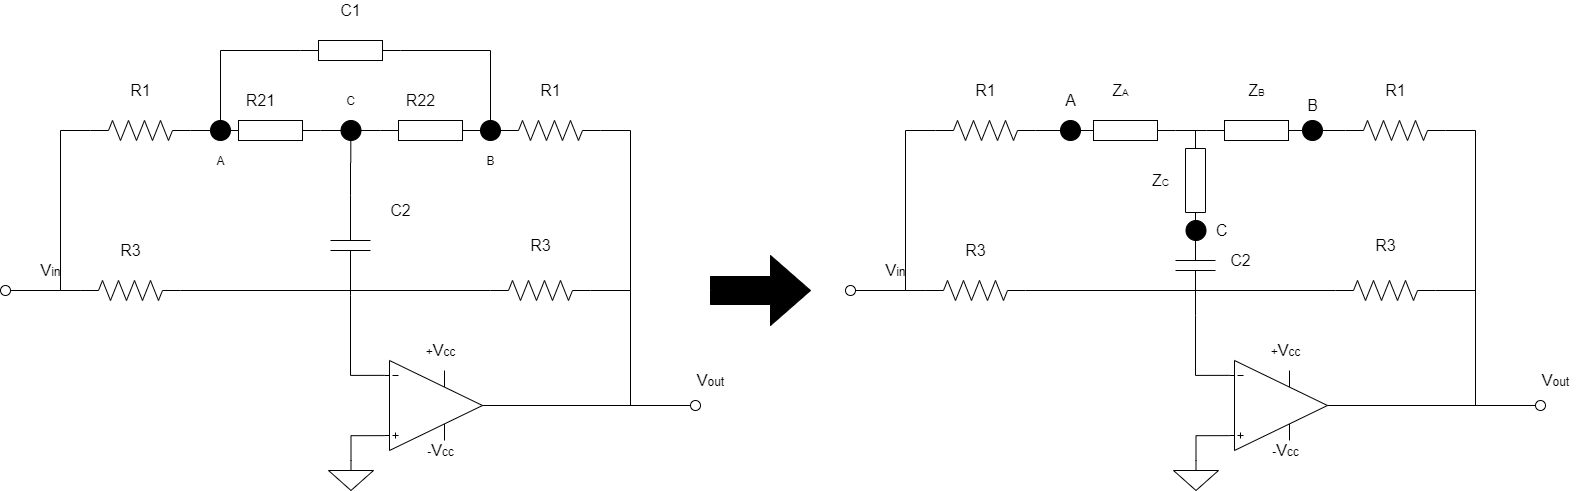
\includegraphics[scale=0.6]{../Ejercicio4-EcualizadorDeFase/Informe/1cambioEstrella.png}
	\label{1reemplazo} 
\end{figure}

Para el segundo reemplazose usaron las siguientes ecuaciones:

\begin{align}
	\begin{equation}
		Z_{A'}= R_1 + Z_{A}
	\end{equation}
	\begin{equation}
		Z_{B'}= R_1 + Z_{B}
	\end{equation}
	
	\begin{equation}
		Z_{C'}= \frac{1}{sC_1} + Z_{C}
	\end{equation}
\end{align}

\begin{figure}[h]
	\caption{2° Reemplazo}
	\centering
	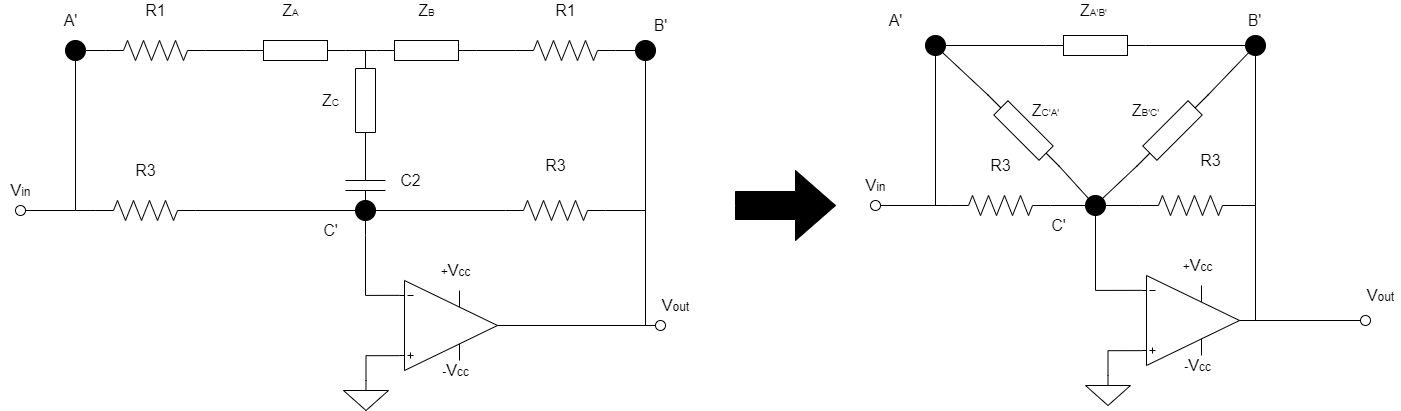
\includegraphics[scale=0.6]{../Ejercicio4-EcualizadorDeFase/Informe/2cambioTriangulo.png}
	\label{2reemplazo} 
\end{figure}

Por último simplificamos las impedancias que estaban en paralelo obteniendo un circuito de 3 impedancias mucho más simple de resolver:

\begin{figure}
	\centering
	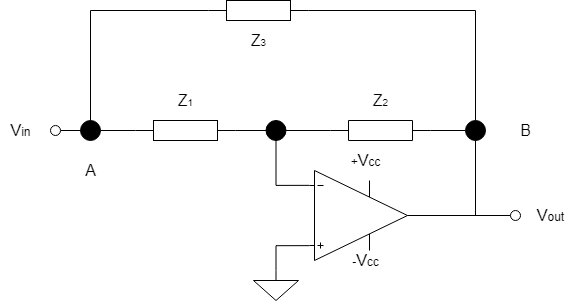
\includegraphics[scale=0.6]{../Ejercicio4_EcualizadorDeFase/Informe/EcFinal.png}
	\caption{Circuito simplificado}
	\label{Cir Final}
\end{figure}

Para no complicar los cálculos se uso el programa Maple para poder obtener los resultados finales de las impedancias.

%%% 	FALTA ALGUNAS ECUACIONES DE IMPEDANCIAS 

\subsubsection{Caso ideal}

Para calcular la transferencia del caso ideal, con las condiciones de $A=\infty $, un $r_{in}=\infty$ y una $r_{out}$ = 0. También se usaron las aproximaciones $C_1 = 10 C_2$, $R_3 >> 1 $ y $R_3 = 10 R_2$ . Luego se procedió a resolver el circuito para obtener la transferencia del circuito de forma ideal. De un simple análisis se puede determinar que:

\begin{align}
	\begin{equation}
		\frac{V_{out}}{Z_2} = \frac{- V_{in}}{Z_1}
	\end{equation}
	
	\begin{equation}
		H(s)=\frac{V_{out}}{V_{in}} = \frac{-Z_2}{Z_1}
	\end{equation}
	\label{ecTransferenciaIdeal}	
\end{align}

%NO SE SI SE PUEDE COMENTAR UN POCO EL RESULTADO

\subsubsection{Caso no ideal}

Si tenemos en cuenta un A finito, con polo dominante, un $r_{in}$ finito y una $r_{out}$ = 0, refiriéndonos de esta forma a un caso que se asemeja más a un modelo real, teniendo en cuenta que se consideran más factores para aproximar a las condiciones reales del circuito. Así el circuito funcionara con la respectiva salida

\begin{align}
	
	\begin{equation}
		H(s)=\frac{V_{out}}{V_{in}} = \frac{s^2 \alpha + s \gamma_z + \beta}{s^2 \alpha + s \gamma_p + \beta}
	\end{equation}
	\label{ecTransferencia}
	
	\begin{equation}
		\alpha= 
	\end{equation}
	
	\begin{equation}
		\beta= 
	\end{equation}
	
	\begin{equation}
		\gamma_z= 
	\end{equation}
	
	\begin{equation}
		\gamma_p= 
	\end{equation}
	
\end{align}


Para facilitar escribir la ecuación se usaron los reemplazos ya mostrados. De la ecuación \ref{ecTransferencia} se puede determinar que la frecuencia de corte del circuito es:


\begin{align}

	\begin{equation}
		\omega_0 = \sqrt{\frac{\beta}{\alpha}}
	\end{equation}
	
	\begin{equation}
		f_0 = \frac{1}{2\pi} . \sqrt{ \frac{2R_1 + R_2 }{ 20 C_2^2 R_1 R_2^2 (L (1-L)) + 100R_1 R_2^2C_2^2 } }
	\end{equation}
	
	\begin{equation}
		f_0 = \frac{1}{2\pi C_2 R_2} \sqrt{ \frac{2 + \frac{R_2}{R_1} }{ 20L(1-L) + 100 } }
	\end{equation}		
	\label{f0sinsimplificar}
	
	\begin{equation}
		f_0 = \frac{1}{2\pi C_2 R_2} \frac{ \sqrt{ \frac{2 + \frac{R_2}{R_1} }{ 1 } } }{ 10 }
	\end{equation}
	\label{f0final}
	
\end{align}

\subsubsection{•}